\subsection{Availability}
    
As we mentioned in the introduction to this chapter, the datasets may be available in the original source. However, this doesn't necessarily
mean that they are readily accessible.
The challenges we encounter with the raw data direct from the source of origin, are the following: \\   
 
\textbf{Location}. Datasets are usually available in open data portals that have been organized and structured in particular ways.
Despite more companies attempting to offer functional and efficient user interfaces, often a complicated search and selection process is necessary for a user to find what they need. Sometimes the data may not all be available in the one location, but may require searching through multible portals.
\textbf{Extraction}. Datasets are usually available through an API (Application Programming Interface). APIs are not easily interpretable by the average user. Normally there will be a document describing the fields and values presented, and indicating how to actually use the API. \\

\textbf{Readability}. Datasets are usually represented in a format designed to be processed by software. This is fairly unintelligible to a human user. At best,
the data will be represented in a table and even then, it will often be quite difficult to extract the required information.

Therefore, we can not say that data interfaces are commonly accessible in a useful way for the average user. \\

\subsubsection{How can we solve the problem?} 

We must provide the information required by the user in an uncomplicated manner, in a format that is easy to read and interpret, and we must describe it in a way that is easy to understand and quick to digest..

In order to collect the information which is relevant to the user, we will need to carry out processes such as extraction, transformation and
data cleaning.
 
\subsubsection{How we solve it using Aire Guru.} 

Our tool uses the air quality data provided by the city of Málaga in its open data portal.(https://datosabiertos.malaga.eu/)\\
\begin{figure}[ht]
    \centering
   \subfigure[Main page]
    {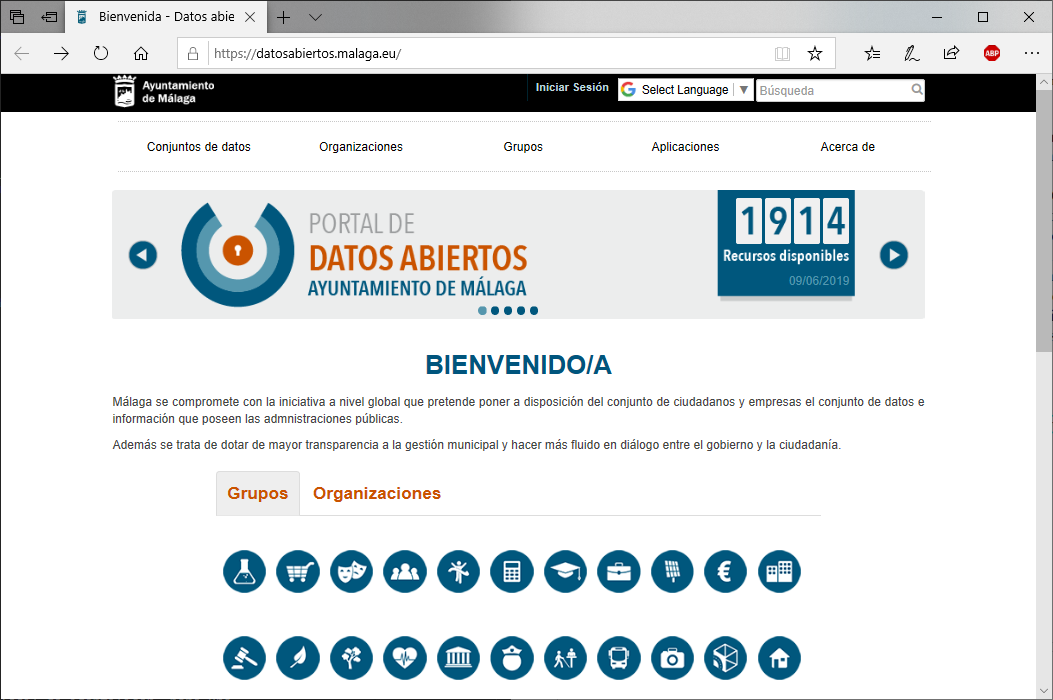
\includegraphics[width=5.5cm]{openDataPortal}}
    \hfill
    \subfigure [Category environment]
       { 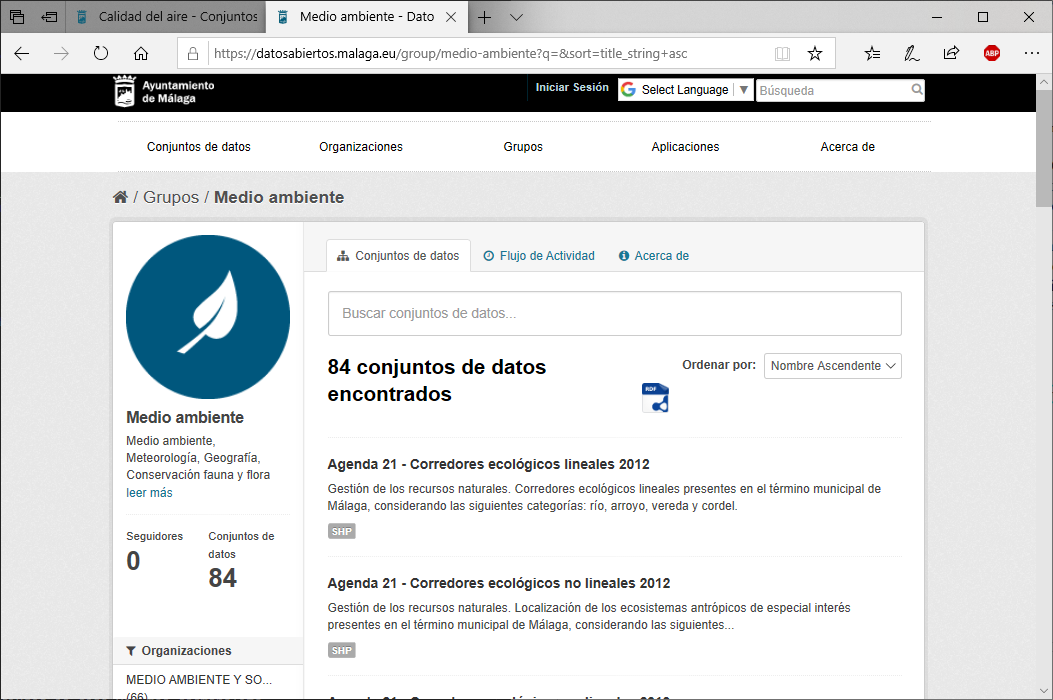
\includegraphics[width=5.5cm]{openDataPortalEnviromentCategory}}




    \vfill
     \subfigure[GeoJson Document]
     { \centering 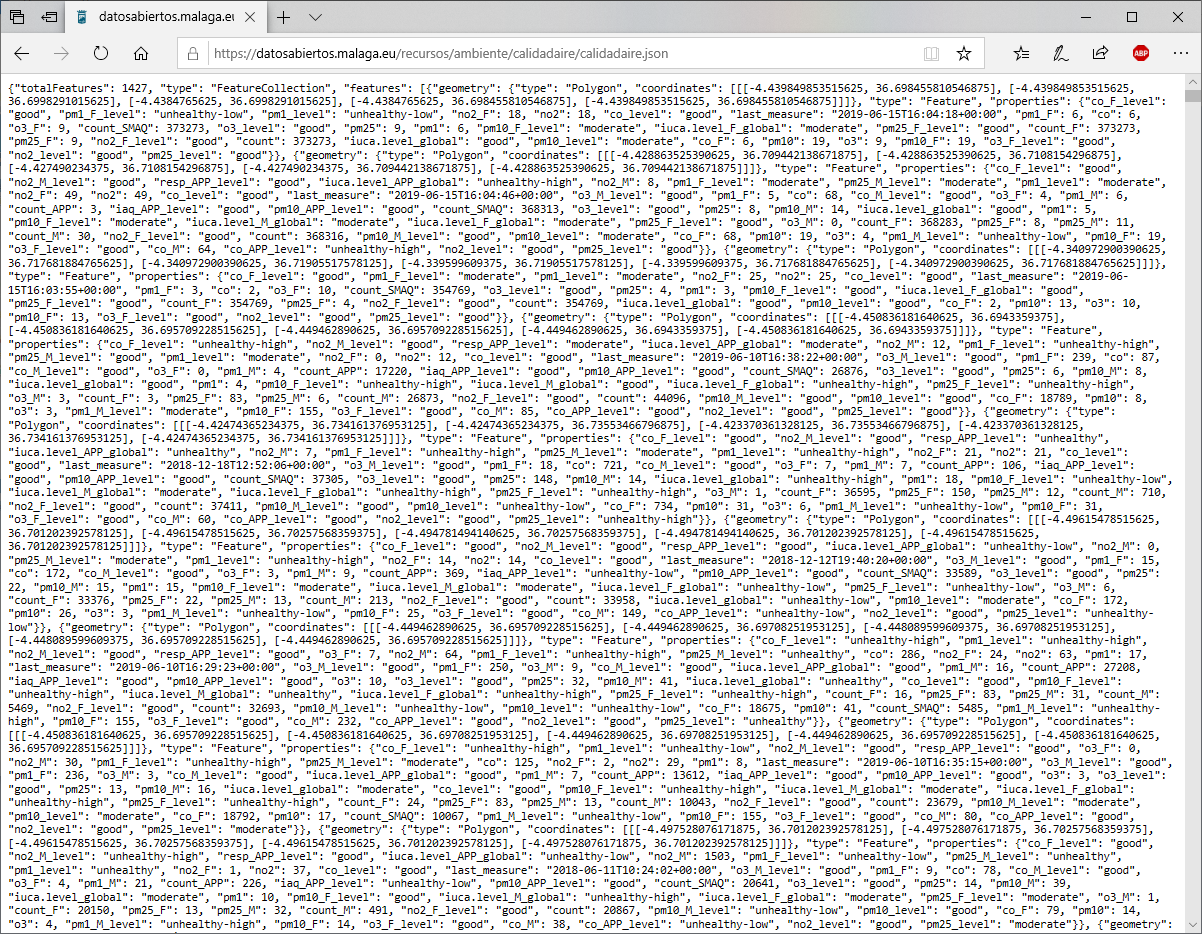
\includegraphics[width=4.75cm]{geoJsonAirQualityDataRaw}}
  
  \caption{Open Data Portal Málaga}
    \end{figure}

    This data portal offers a variety of categories (represented by different icons) indicating classifications of the dataset.
    Once a category is selected, the user is presented with a search bar that allows them to search for specific data using keywords.\\
    
    In this case, if we click on the link, data is displayed in a new tab. The use of software
    for translating the data is not strictly necessary, but we can see that the format (JSON) is not easily readable in human terms.

Aire Guru (https:\\aire.guru) offers all the necessary information on a web platform which has been designed to facilitate human understanding.

\elsparagraph{Evaluation}  

\begin{itemize}
    \done Location. Finding data is made simple, since information is displayed immediately on accessing the website. The main page
         presents the levels of pollution in all areas without the need to make any selection.
    \done Extraction. No specialist software or computer knowledge is necessary to access the information.
    \done Readability. Aire Guru includes a map which shows pollution levels, represented by different colors. These colors are defined by a legend
         below the map. It also includes a glossary explains the concepts presented on the website, the meaning of each section and includes clear instructions on how to
         use and navigate through the web page.
 

\end{itemize}
\newpage

 


